\chapter{Testprozess}
\label{testentwurf}

Nachdem festgestellt wurde, dass die PrimePfad Abdeckung potenziell das sinnvollste Abdeckungskriterium ist, soll im Folgenden eine
Methodik entwickelt werden, die es erlaubt, mithilfe des Abdeckungskriteriums Tests für GraphQL zu entwerfen.
Die zu entwickelnde Methodik wird in einigen Teilen stark an der Methode aus~\cite{property-based-testing} orientiert sein, das ist jedoch an den betreffenden Stellen kenntlich gemacht.
In diesem Kapitel wird die Methodik konzeptionell erstellt und im folgenden Kapitel~\ref{testautomatisierung} ein Prototyp entwickelt, der
die Methodik umsetzt und validiert.
Die zu entwickelnde Methode arbeitet grob nach dem in Abbildung~\ref{methodeablauf} gezeigten Muster.

\begin{figure}[H]
    \centering
    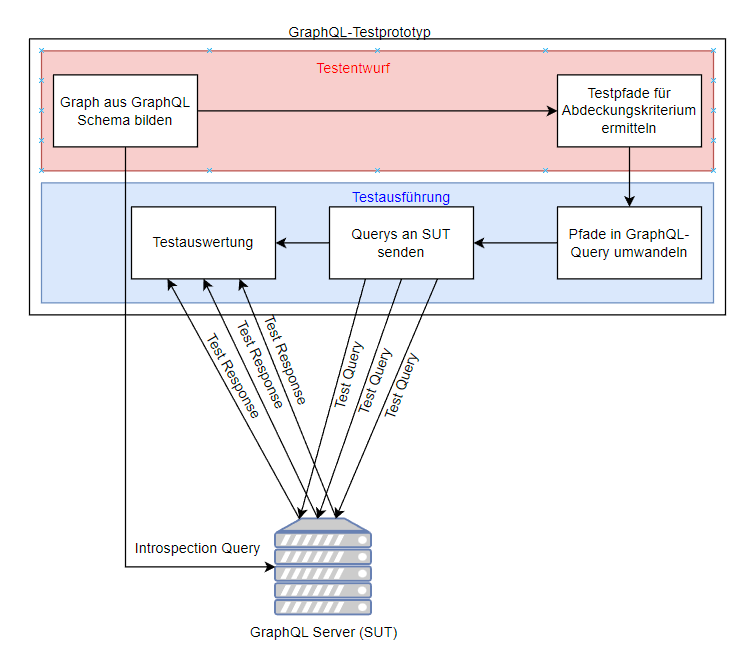
\includegraphics[width=0.75\textwidth,keepaspectratio]{img/fktweiseprototyp}
    \caption{Grober Ablauf des Testprozesses}
    \label{methodeablauf}
\end{figure}

Wie in Abbildung~\ref{methodeablauf} zu sehen, ist der gesamte Testprozess in zwei Teile aufgeteilt.
Einerseits in den Testentwurf, andererseits in die Testausführung.
Der Testentwurf basiert auf den zuvor erarbeiteten Theorien und die Testausführung orientiert sich stark am
Property-based Testing~\cite[vgl. Method]{property-based-testing}.

\section{Testentwurf}
\label{testentw}
Der erste Abschnitt des Testprozesses erarbeitet die Pfadgenerierung nach gewähltem Abdeckungskriterium.
Wie zuvor festgestellt, wird die PrimePfad Abdeckung im Folgenden ermittelt.
Die Methode erlaubt allerdings auch einen Wechsel des Abdeckungskriteriums, da im Endeffekt nur die Pfade für die weiteren Prozesse
genutzt werden können.
Bevor jedoch ein Abdeckungskriterium genutzt werden kann, muss das GraphQL-Schema in einen Graphen übersetzt werden.

\subsection{GraphQL-Schema in Graph abbilden}
\label{schemagraph}

Laut GraphQL-Specification~\cite{graphqlspecification} erlaubt ein GraphQL Server, dass Abfragen über die Schemastruktur des
Servers erlaubt sind~\cite[vgl. 4. Introspection]{graphqlspecification}.
Mithilfe der Introspection-Query~\ref{introspection-query} lässt sich das gesamte Schema eines GraphQL-Servers abrufen.
Die Introspection-Query existiert in verschiedenen Varianten.
Hier wird die exakt gleiche Version genutzt, wie sie auch von~\cite{property-based-testing} verwendet wird.
Ergebnis der Introspection Query ist ein JSON-Objekt mit einer Struktur wie in Listing~\ref{introspec} gezeigt.

\begin{lstlisting}[language=json, caption={Schema-Response},captionpos=b]
    {
        "data": {
            "__schema": {
                "queryType": {},
                "mutationType": {},
                "subscriptionType": {},
                "types": [],
            }
        }
    }
\end{lstlisting}
\label{introspec}

Der Eintrag $queryType$ gibt den Namen des Typens an, der Startpunkt jeder Query ist, so wie in Kapitel~\ref{gqlcov} festgelegt.
Im Eintrag $types$ ist eine Liste aller Typen enthalten, wobei jeder Eintrag der Struktur im Listing~\ref{typstrukt} entspricht.

\begin{lstlisting}[language=json, caption={Type-Field},captionpos=b]
        {
          "kind": "",
          "name": "",
          "description": "",
          "fields": [],
          "inputFields": [],
          "interfaces": [],
          "enumValues": [],
          "possibleTypes": []
        }
\end{lstlisting}
\label{typstrukt}


Um aus dem Schema einen Graphen zu erstellen, werden die Felder $kind$, $name$ und $fields$ benötigt.
Die Angabe $kind$ gibt an, von welchem Typ das Feld ist.
Hierbei gibt es 9 Möglichkeiten, die dieses Feld annehmen kann.

\begin{itemize}
    \item \textbf{ObjectTypeDefinition (OBJECT):} Repräsentiert ein Objekt mit Feldern.
    \item \textbf{ScalarTypeDefinition (SCALAR):} Eingebaute oder benutzerdefinierte Typen wie \texttt{Int}, \texttt{Float}, \texttt{String}, \texttt{Boolean} und \texttt{ID}.
    \item \textbf{InputObjectTypeDefinition (INPUT\_OBJECT):} Erlaubt das Übergeben komplexer Objekte als Argumente.
    \item \textbf{InterfaceTypeDefinition (INTERFACE):} Repräsentiert eine Liste von Feldern, die andere Objekttypen enthalten müssen.
    \item \textbf{UnionTypeDefinition (UNION):} Kann einen von mehreren Arten von Objekttypen repräsentieren.
    \item \textbf{EnumTypeDefinition (ENUM):} Ein Skalartyp, der auf eine bestimmte Liste von Werten beschränkt ist.
    \item \textbf{ListTypeDefinition (LIST):} Repräsentiert eine Liste von Werten eines bestimmten Typs.
    \item \textbf{NonNullTypeDefinition (NON\_NULL):} Ein Modifikator, der angibt, dass der angewandte Typ nicht null sein kann.
    \item \textbf{DirectiveDefinition (DIRECTIVE):} Passt das Verhalten von Feldern oder Typen des Schemas an.
\end{itemize}

Aus allen Feldern des Typen $OBJECT$ kann ein Graph gebildet werden.
Die Menge aller Objekte vom Typ $OBJECT$ ist die Menge aller Knoten des Graphens.
Kanten werden dem Graphen hinzugefügt indem die einzelne Typdefinition näher betrachtet wird.
Wie in $Type-Field$ gesehen, definiert ein Type immer ein Feld $fields$.
In diesem Feld $fields$ verbirgt sich die Informationen aller Kanten, die ausgehend von diesem Knoten sind.
Das Feld $fields$ beeinhaltet Objekte folgender Struktur:

\begin{lstlisting}[language=json, caption={Type-Field},captionpos=b]
            {
              "name": "",
              "description": "",
              "args": [],
              "type": {},
              "isDeprecated": "",
              "deprecationReason": ""
            }
\end{lstlisting}

Wobei für die Ermittlung der Kanten das Feld $type$ besonders wichtig ist.
Das Feld ist nach Schema aus Listing~\ref{typefiel} definiert.

\begin{lstlisting}[language=json, caption={Type-Field},captionpos=b, label={typefiel}]
    {
        "kind": "",
        "name": "",
        "ofType": null
    }
\end{lstlisting}

Wenn der Eintrag $kind$ den Wert $OBJECT$ trägt, so ist klar, dass das hier definierte $OBJECT$ eine Kante zum Knoten $name$ besitzt.

\subsection{PrimePfade ermitteln}
\label{testpfade}

Aus dem zuvor ermittelten Graphen sollen Testpfade ermittelt werden, welche die PrimePfad-Abdeckung erfüllen.
Hierzu wird der in~\cite[Finding Prime Test Paths]{software-testing} vorgestellte Algorithmus genutzt.
Dabei werden zuerst die einfachen Pfade ermittelt und dann gefiltert.
Dies sind Pfade ähnlich zu Definition~\ref{primepfad} mit der Lockerung, dass diese Pfade auch Teilpfad eines längeren Pfads sein können~\cite[vgl. S. 35]{software-testing}.
Der längste einfache Pfad kann maximal so lang sein wie die Anzahl der Knoten des Graphens~\cite[vgl. S.41 ]{software-testing}.
Es wird von jedem Knoten aus expandiert und eine Liste über alle Pfade geführt.
Pfade werden nicht weiter expandiert, wenn diese einen Knoten doppelt enthalten.
Das Endergebnis ist dann eine Liste aller einfachen Pfade.
Diese Liste wird gefiltert, indem alle Pfade, die Teilpfad eines anderen Pfads sind, verworfen werden.
Nach Definition~\ref{primecov} wird so die PrimePfad-Abdeckung erlangt.
Dies folgt, da die Menge der PrimePfade eine echte Teilmenge der einfachen Pfade ist~\cite[vgl. S. 35]{software-testing}.
Mit der Einschränkung von GraphQL, dass valide Queries stets im Query-Knoten starten müssen, muss sichergestellt werden, dass die PrimePfade dort starten.
Um dies umzusetzen, wird festgelegt, dass der kürzeste Weg vom Query Knoten zum Startknoten des PrimePfades zu ermitteln ist und an den PrimePfad anzuhängen,
sodass aus diesem später eine valide Query generiert werden kann.
Es lässt sich also festhalten, dass zuerst die Pfade für eine PrimePfad Abdeckung berechnet werden müssen
und diese dann zu gültigen Testpfaden erweitert werden sollen, sodass sie GraphQL Konventionen einhalten.

\newpage
\section{Testausführung}

Die ermittelten Pfade werden zu validen GraphQL-Queries umgewandelt und dann ausgeführt um den Test zu validieren.
Die Pfadumwandlung in eine valide Query ist noch methodisch stark abweichend zu~\cite{property-based-testing}.
Spätere Schritte, also Test ausführen und auswerten sind methodisch gleich zu~\cite{property-based-testing}.

\subsection{Pfade in Query umwandeln}
\label{pfadquery}

Die Umwandlung eines Pfads in eine Query erfolgt durch die Verwendung der Typinformationen aus dem GraphQL-Schema.
Der Pfad wird beginnend im Query-Knoten abgelaufen.
Das GraphQL-Schema enthält Informationen darüber, welche Informationen nötig sind, um zum nächsten adjazenten Knoten des Pfads zu kommen.
Die Informationen darüber sind im Eintrag $fields$ enthalten, wie in Listing~\ref{typstrukt} gesehen.
Im $fields$ Eintrag steht, ob eine Kante Argumente benötigt und welchen Typ das Rückgabeobjekt hat.
Das Rückgabeobjekt des $fields$ steht dabei aber schon fest, da dieser exakt gleich sein muss mit dem nächsten Knoten des Pfads.
In jedem Schritt der Query-Generierung werden stets alle Felder vom Typ $SCALAR$ hinzugefügt, damit sichergestellt werden kann, dass
der Typ alle Felder implementiert hat.
Je nach Implementierung können durch die Feldauswahl weitere Funktionen abgefragt werden, daher ist alles zu inkludieren.
Felder vom Typ $OBJECT$ werden nur zur Query hinzugefügt, wenn der Typ des $OBJECT$ dem nächsten Knoten entspricht.
Im Allgemeinen lässt sich das Verfahren durch den Pseudocode in Listing~\ref{pfadgen} darstellen. \\

\begin{lstlisting}[caption={Pseudocode für Pfadgenerierung},captionpos=b, label={pfadgen}]
    path = (A , B , ..... , Y)
    query = {}

    while path not empty:
        knoten = pfad.pop()
        ScalarFields = getScalarFields(knoten)
        query.addScalars(ScalarFields)
        edge = pfad.peek()
        args = checkForEdgeArgs(edge)
        query.addArgs(args)
    return query
\end{lstlisting}

Die Argumente, die in einer Query verwendet werden, sind stets nur $SCALAR$ Types und somit einfache Datentypen.
Es gibt verschiedene Arten die Argumentgeneratoren umzusetzen, vorerst werden diese jedoch methodisch exakt wie in~\cite{property-based-testing} umgesetzt.
Dabei wird der Typ des Arguments genutzt, um zufällig ein Argument des entsprechenden Datentyps zu generieren.
Ergebnis des Prozesses ist schließlich eine valide GraphQL-Query.
In einer konkreten Implementierung ist die Syntax von GraphQL zu beachten, diese ist einsehbar in~\cite[2.3 Language Operations]{graphqlspecification}.

\subsection{Queries an Server senden}
\label{testf}

Die generierten Queries stellen die konkreten Tests für den GraphQL-Server dar.
Im Folgenden wird der GraphQL-Server vermehrt SUT (System under Test) genannt.
Eine Auswertung der Tests geschieht, indem alle generierten Queries per HTTP-POST an den GraphQL-Server geschickt werden.
Die gelieferten Antworten sind zu speichern, dies ist analog zu~\cite{property-based-testing}.
Es ist wünschenswert, dass die generierten Queries in einem Testframework abgebildet und gespeichert werden.
Dadurch werden die Tests reproduzierbar und können später verwendet werden, um etwaige Fehlerbehebungen zu verifizieren.

\subsection{Testauswertung}

Die Auswertung der Tests basiert auf denselben Annahmen, wie sie in~\cite{property-based-testing} getroffen wurden.
Dabei werden die HTTP-Codes der Antworten (im folgenden oft Response) und die existierenden Keys in der Response überprüft.
Eine Antwort eines GraphQL-Servers liefert stets einen Statuscode \textbf{200}, wenn kein kritischer Fehler auftrat.
Kritische Fehler sind stets ein Statuscode \textbf{500}~\cite[vgl. 7. Response]{graphqlspecification}.
Daher wird jede Antwort mit einem Code \textbf{500} als gefundener Fehler und fehlerhafter Test betrachtet.
Eine Antwort mit einem Statuscode \textbf{200} kann jedoch auch Fehler aufweisen.
Dies wird ersichtlich durch einen zweiten Haupteintrag $errors$ in einer Antwort, ersichtlich in Listing~\ref{err}.

\begin{lstlisting}[language=GraphQL, label={err}, caption={fehlerhafte Antwort}]
    {
        "data": {}
        "errors": {}
    }
\end{lstlisting}

Die Einträge in $errors$ müssen jedoch manuell geprüft werden, ob es sich um einen wirklichen Programmierfehler handelt oder gewünschtes Verhalten,
da die Zufallsargumente teilweise dafür sorgen, dass Konventionen nicht eingehalten werden können.
Die Zufallsargumente sorgen allerdings auch dafür, dass die errechnete PrimePfad Abdeckung nicht praktisch erreicht wird.
Sehr häufig kommt es vor, dass zufällig generierte Argumente schon in den Anfängen des Pfads nicht passend zu den vorhandenen Daten sind.
Dadurch folgt, dass ein Großteil der Testpfade, die theoretisch eine gute Abdeckung aufweisen, praktisch diese Abdeckung nicht erreicht.
Um messen zu können, ob ein Pfad seine theoretische Abdeckung auch praktisch erreicht, wird eine Abschätzung eingeführt.

\subsubsection{Abschätzung der Pfadlängen}

Mit einer Abschätzung werden die Testergebnisse nicht besser, allerdings können so Informationen darüber gewonnen werden, wie viel
vom getesteten Pfad tatsächlich abgedeckt wurde.
Dadurch lässt sich der Erfolg der Tests besser abschätzen, da so messbar wird, ob die Queries wirklich die Funktionen ausgeführt haben.
Hierzu wird die Pfadlänge des Pfads, der zur Erstellung der Query genutzt wurde, als erwartete Pfadlänge angenommen.
Die Pfadlänge der Antwort wird dann als tatsächliche Pfadlänge genommen.
Der Unterschied zwischen erwarteter und tatsächlicher Pfadlänge ist dann das Auswertungsmerkmal für diesen speziellen Test.
Die Pfadlänge der Response ist die maximale Tiefe der JSON-Response verringert um 1.

\[ \text{Tiefe des Pfades} = \text{Tiefe des JSON-Response-Objekts} - 1 \]

Demnach hat die Response aus Listing~\ref{resp3} eine Tiefe von 2.

\begin{lstlisting}[language=GraphQL, caption={vollständige Response}, label={resp3}]
    {
        "data": {
            "book": {
                id: "1",
                title: "Moby Dick"
                publisher: {
                    id: "1",
                    name: "Testverlag"
                }
            }
        }
    }
\end{lstlisting}

Eine leere Antwort, wie in Listing~\ref{resp4} gezeigt, hat eine Tiefe von 1.

\begin{lstlisting}[language=GraphQL, caption={mangelhafte Response}, label={resp4}]
    {
        "data": {
            "book": null
        }
    }
\end{lstlisting}

Obwohl eine leere Response zulässig ist und nicht direkt auf einen Fehler hindeutet, signalisiert der Unterschied zwischen erwarteter und tatsächlicher Länge,
ob die Query tatsächlich alle Resolver ausgeführt hat oder nur einen Teil davon.
Mithilfe der Abschätzung kann die Qualität der Tests ausgewertet werden.
Hierzu kann die Pfadlänge aller erwarteten Pfade addiert werden.
Das gleiche wird mit den tatsächlichen Pfadlängen gemacht.
Beide Zahlen können dann miteinander in Bezug gesetzt werden, um eine prozentuale Einschätzung zu erlangen, wie viel Prozent der Tests
tatsächlich ausgeführt wurden.
\begin{definition}
    \[ \text{Prozent der tatsächlichen Abdeckung} = \frac{\text{tatsächliche Gesamtpfadlänge}}{\text{erwartete Gesamtpfadlänge}} * 100 \]
\end{definition}

Ein Wert von 100\% ist anzustreben.
Dies würde bedeuten, dass die generierten Tests auch alle Funktionen getestet haben.
In der Praxis wird der Wert jedoch sehr wahrscheinlich darunter liegen.
\\
\\

Abschließend soll erklärt werden, wie es möglich ist, den Wert der tatsächlichen Abdeckung zu erhöhen.
Dies geschieht durch zwei verschiedene Methoden.

\subsubsection{Zufallsgeneratoren der Argumente}
\label{zufallsgen}

Die zuvor vorgestellte Abschätzung liefert einen Hinweis darüber, wie gut die Queries tatsächlich getestet wurden.
Ein Ansatz, der die Queries eine bessere tatsächliche Abdeckung erreichen lässt, ist das Anpassen der Generatoren für die Argumente.
Bei der in Kapitel~\ref{pfadquery} vorgestellten Methode werden Argumente komplett zufällig für den zugrundeliegenden Datentyp erstellt.
Dies bedeutet, dass zum Beispiel der Type $ID$ als String gewertet wird.
Eine $ID$ unterliegt jedoch in den allermeisten Implementierungen bestimmten Konventionen.
So wäre ein Generator für zufällige Strings nicht in der Lage, solche Konventionen zuverlässig abzubilden.
Ein Anpassen des Argumentgenerators für die $ID$ an die verwendete Konvention des SUT hilft dabei, dass signifikant bessere Ergebnisse erzeugt werden.
Alternativ kann auch eine Liste aller existenten IDs angegeben sein und zufällig ein Element ausgewählt werden.
Die Anpassung der Argumentgeneratoren an die zugrundeliegenden Daten ist höchst spezifisch und daher kann keine allgemeine
Vorgehensweise ermittelt werden.
Ziel der Anpassung ist es, dass die Chance erhöht wird, dass Argumente zufällig generiert werden, die dann tatsächlich zu den zugrunde liegenden Daten passen.

\subsubsection{Anzahl der Queries}

Die Wahrscheinlichkeit, passende Argumente zu generieren, steigt mit der Anzahl an generierten Queries.
Wird die Anzahl an generierten Queries pro Pfad erhöht, so steigt auch die Wahrscheinlichkeit, dass zumindest ein Pfad eine gute Abdeckung erreicht.
Hierfür muss die Methode aus Kapitel~\ref{pfadquery} so oft wie gewünscht wiederholt werden.
In jeder Generierung muss jedoch das Ergebnis sein, dass verschiedene Argumente für die Query generiert wurden.
Zusammen mit den angepassten Argumentgeneratoren kann so die zufallsbasierte Argumentgeneration begrenzt werden
und es ist wahrscheinlicher, dass gute Tests entstehen.


\section{Zusammenfassung der Methode}

Die eben entwickelte Methode funktioniert so wie in Abbildung~\ref{methodeablauf} gezeigt.
Teile der Methode bedienen sich an Methoden die in~\cite{property-based-testing} eingeführt wurden.
Der komplette Prozess der Testgenerierung wurde in der hier entwickelten Methode jedoch verändert.
So wurde die Graphstruktur von GraphQL genutzt, um aus dieser Testpfade zu generieren, die dann in GraphQL-Queries umgewandelt werden.
Auf diese Weise war es möglich, die Limitierung des Rekursionslimits vom \textit{Property-based Testing} zu beseitigen.
In der Testauswertung wurde sich stark am \textit{Property-based Testing} orientiert.
Die Einführung der erwarteten Pfadlänge gegenüber der tatsächlichen Pfadlänge ist ein neuer Ansatz, der die Qualität der zu testenden Queries
messbar macht.
Das fehlt im \textit{Property-based Testing} .
\\


Im Folgenden soll die entwickelte Methode in einem Prototypen umgesetzt werden.
Dieser Prototyp soll dann in Experimenten zeigen, dass die entwickelte Methode in der Lage ist, Fehler in GraphQL-APIs zu finden.
Ein Vergleich mit dem Prototypen von \textit{Property-based Testing} soll zeigen, ob die Methode Verbesserungen bringt.







